%%%%%%%%%%%%%%%%%%%%%%%%%%%%%%%%%%%%%%%%%
% FRI Data Science_report LaTeX Template
% Version 1.0 (28/1/2020)
% 
% Jure Demšar (jure.demsar@fri.uni-lj.si)
%
% Based on MicromouseSymp article template by:
% Mathias Legrand (legrand.mathias@gmail.com) 
% With extensive modifications by:
% Antonio Valente (antonio.luis.valente@gmail.com)
%
% License:
% CC BY-NC-SA 3.0 (http://creativecommons.org/licenses/by-nc-sa/3.0/)
%
%%%%%%%%%%%%%%%%%%%%%%%%%%%%%%%%%%%%%%%%%


%----------------------------------------------------------------------------------------
%	PACKAGES AND OTHER DOCUMENT CONFIGURATIONS
%----------------------------------------------------------------------------------------
\documentclass[fleqn,moreauthors,10pt]{ds_report}
\usepackage[english]{babel}

\graphicspath{{fig/}}




%----------------------------------------------------------------------------------------
%	ARTICLE INFORMATION
%----------------------------------------------------------------------------------------

% Header
\JournalInfo{FRI Natural language processing course 2025}

% Interim or final report
\Archive{Project report} 
%\Archive{Final report} 

% Article title
\PaperTitle{Conversational Agent with Retrieval-Augmented Generation for research assistance} 

% Authors (student competitors) and their info
\Authors{Marko Medved, Sebastijan Trojer, and Matej Vrečar}

% Advisors
\affiliation{\textit{Advisor: Aleš Žagar}}

% Keywords
\Keywords{Retrieval augmented generation, research assistance, re-identification}
\newcommand{\keywordname}{Keywords}


%----------------------------------------------------------------------------------------
%	ABSTRACT
%----------------------------------------------------------------------------------------

\Abstract{
Large language models (LLMs) are increasingly used in conversational agents for academic support, but they often struggle with outdated knowledge and hallucinations in specialized domains. To address this, we developed a conversational assistant using Retrieval-Augmented Generation (RAG), focusing on the field of automatic re-identification. Our system retrieves recent research papers from arXiv and CVF, processes them using domain-adapted query rewriting and relevance-based re-ranking, and integrates this context into language model responses. We implemented and evaluated both a baseline and an attempt of
 an improved retrieval pipeline, emphasizing relevance over exact matches. 
% TODO results
}

%----------------------------------------------------------------------------------------

\begin{document}

% Makes all text pages the same height
\flushbottom 

% Print the title and abstract box
\maketitle 

% Removes page numbering from the first page
\thispagestyle{empty} 

%----------------------------------------------------------------------------------------
%	ARTICLE CONTENTS
%----------------------------------------------------------------------------------------

\section*{Introduction}
LLMs have become increasingly capable in natural language understanding and generation, making them attractive for use in academic research support. However, their utility is limited by knowledge cutoffs and susceptibility to hallucinations, particularly in fast-evolving or specialized fields. To address these limitations, we developed a conversational assistant based on RAG, targeting the domain of person re-identification—a challenging task in computer vision.

Our system combines a pretrained language model with a retrieval pipeline that fetches recent research papers from sources like arXiv and CVF. The goal is to provide accurate, up-to-date answers by integrating external knowledge into the model's responses. In this project, we emphasize improvements to the retrieval process, which is critical for maximizing the relevance and utility of generated responses, by providing relevant context.

We implemented both a baseline and an enhanced retrieval pipeline. The latter includes query rewriting, domain-specific filtering, and re-ranking strategies aimed at improving contextual relevance. Evaluation focues on the system's ability to retrieve relevant papers and generate accurate responses to academic queries, particularly those related to recent developments in automatic re-identification. We compare the performance of our baseline RAG system with the enhanced pipeline, assessing retrieval effectiveness using metrics inspired by Cumulative Matching Characteristic (CMC) and mean Average Precision (mAP).




%------------------------------------------------

\section*{Related work}

% Joined

Large Language Models have demonstrated strong language understanding and generation capabilities, but they often struggle with hallucinations, outdated knowledge, and limited domain-specific accuracy, especially when handling specialized research queries~\cite{kandpal2023longtail}. Retrieval-Augmented Generation (RAG) addresses these challenges by enhancing LLMs with real-time information retrieval, improving factual accuracy and relevance~\cite{gao2024rag}. Early RAG models followed a basic retrieve-then-generate structure, but more advanced approaches have introduced techniques like query rewriting, reranking, and adaptive retrieval to improve context relevance and coherence~\cite{gao2024rag}.

Recent research has shown the effectiveness of RAG-based systems for academic and domain-specific applications. For example,~\cite{Chatbots_in_Academia} implemented a RAG system using OpenAI Ada embeddings and GPT-3.5 to enhance information retrieval and synthesis for academic documents, demonstrating the importance of precise embedding strategies for research-based chatbots. Afzal et al.~\cite{afzal2024towards} focused on domain-specific data by creating the CurriculumQA dataset and optimizing retrieval with tailored evaluation metrics such as relevance, coherence, and faithfulness, highlighting the importance of fine-tuning for specific academic fields. Similarly, Yasin et al.~\cite{yasin2024retrieval} integrated advanced techniques—including fine-tuned embedding models, semantic chunking, and abstract-first retrieval—to improve the accuracy and relevance of scholarly content retrieval.

Evaluating RAG systems remains complex due to the nuanced nature of retrieval and generation quality. Chen et al.~\cite{chen2024benchmarking} introduced the Retrieval-Augmented Generation Benchmark (RGB) to measure RAG performance across four key dimensions: noise robustness, negative rejection, information integration, and counterfactual robustness. Their findings show that while RAG improves LLM accuracy, it still struggles with integrating long-distance information and handling noisy or uncertain evidence. Common evaluation methods for RAG systems include retrieval-focused metrics like MRR (Mean Reciprocal Rank) and nDCG (normalized Discounted Cumulative Gain), as well as generation-focused metrics like BLEU and ROUGE to measure the quality and relevance of generated responses~\cite{lewis2020rag}.

In our project, we aim to address these issues by developing a RAG-based chatbot for academic research in automatic re-identification—the task of matching individuals across different cameras or settings, a complex problem in computer vision and machine learning. By focusing on recent research papers from arXiv, we seek to enhance the chatbot’s ability to retrieve and generate accurate responses about the latest developments in automatic re-identification


\section*{Methods}
\subsection*{Baseline}
\subsubsection*{Paper Retrieval from arXiv}
We begin by retrieving candidate papers using the official arXiv API. For each paper, we extract its title, abstract, and metadata. To enable semantic similarity-based filtering, both the user query and the abstracts are embedded using the \textit{allenai-specter} SentenceTransformer model, which is trained to map scientific documents into a dense vector space. We compute cosine similarity between the query embedding and each abstract embedding, and select the top-$k$ most relevant papers ($k=30$ by default).

\subsubsection*{Context Construction}
The titles and abstracts of the top-ranked papers are concatenated into a single text block to serve as external context. This context is inserted into the prompt presented to the language model. No chunking, reranking, or content selection is applied at this stage beyond the similarity-based retrieval.

\subsubsection*{Language Model Inference}
We use \textit{Mistral-7B-Instruct-v0.2} as the language model backend. To enable efficient inference on commodity hardware, the model is loaded using 4-bit quantization with \textit{bitsandbytes}, applying NF4 quantization and bfloat16 compute precision. The model is wrapped with Hugging Face's text-generation pipeline and integrated with LangChain to enable prompt-based question answering. Prompt templates include both the constructed context and the current user query. For comparison, we also evaluate answers generated without any retrieved context.

\subsubsection*{System Behavior}
The system retains a basic conversational memory by concatenating the most recent user query with the current one. This helps preserve short-term context without implementing a full dialogue memory or rewriting mechanism. No fine-tuning is performed, and no re-ranking, filtering, or external knowledge base is used. This baseline is intended to evaluate performance with minimal architectural complexity.


\subsection*{Attempt at an Improved pipeline for retrieval}

A modified RAG system was implemented to explore potential improvements in relevance and accuracy for person re-identification from video. The updated pipeline introduces several architectural changes aimed at more targeted retrieval and domain-aligned generation:

\begin{itemize}
    \item \textit{Two-stage query rewriting}: Queries are rewritten separately for retrieval (search) and semantic matching, allowing distinct optimization for recall and ranking.

    \item \textit{Domain-specific augmentation}: Rewritten queries are enriched with terms such as \textit{person re-identification} and restricted to the \textit{cs.CV} category to better focus the search on relevant literature.

    \item \textit{Local database integration}: A local CVF paper database supplements arXiv results, expanding the overall coverage of relevant academic sources.

    \item \textit{Unified re-ranking}: Retrieved documents are encoded using \textit{allenai-specter} and re-ranked via cosine similarity against the match-stage query.

    \item \textit{Task-specific prompting}: Prompts used during response generation are tailored for the Re-ID task to better align outputs with domain-specific needs.
\end{itemize}

Figure~\ref{fig:retrieval_pipeline} presents an overview of the enhanced 
pipeline, including the two-stage query rewriting, integration of a
 local CVF database, and re-ranking strategy. These modifications were 
 evaluated against the baseline architecture, with comparative analysis 
 focusing on retrieval relevance.


\begin{figure*}[h]
    \centering
    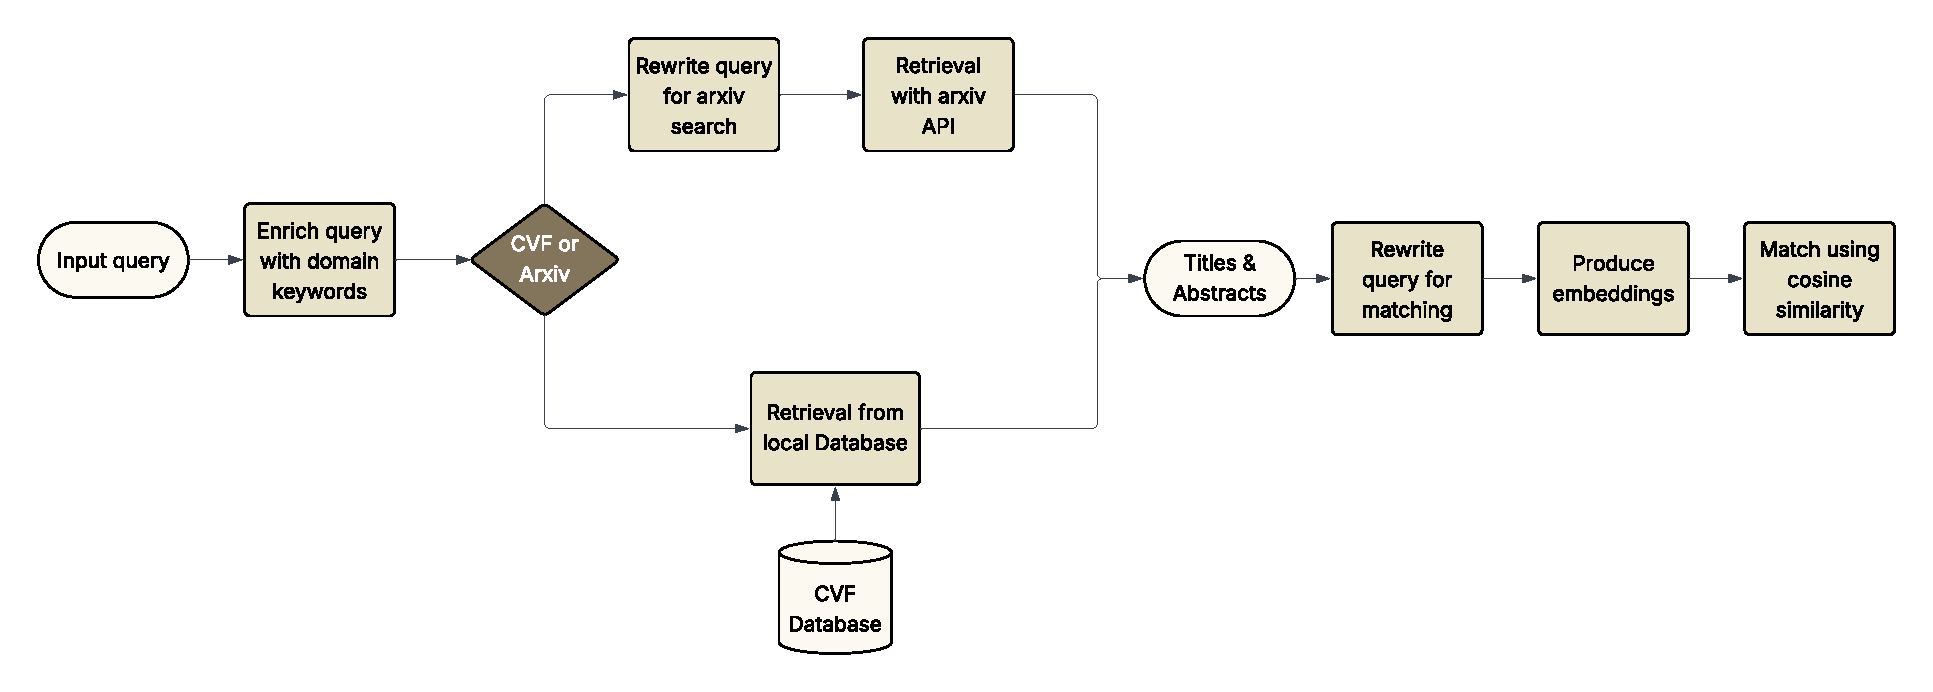
\includegraphics[width=\textwidth]{fig/flowchart.pdf}
    \caption{Overview of the enhanced retrieval pipeline.}
    \label{fig:retrieval_pipeline}
\end{figure*}







\section*{Preliminary results }
To evaluate the effectiveness of our RAG-enhanced approach, we tested it on scientific
 questions related to papers published after December 2023. The goal was to determine 
 whether the system could incorporate recent research not seen during the original
  model’s training.

Across a range of prompts, results showed that while the system often failed to retrieve 
the exact target paper with top-$k=5$, it still produced more informative and current responses by leveraging similar recent articles. Increasing $k$ to 10 improved retrieval in several cases—for example, retrieving a nearly identical sentiment analysis paper by the same authors.

Refined queries also led to improved results. For a fast and robust covariance estimator, adding terms like “low contamination regime” and “near-linear sample complexity” helped surface the correct article. In contrast, generic queries often led the model to irrelevant domains, such as quantum mechanics.

For topics like NP-complete problems and object detection, specificity again proved critical. While exact matches were rare, the RAG system offered responses more reflective of recent research trends than the baseline. However, it occasionally exhibited erratic behavior, such as generating its own sub-questions, which significantly increased inference time.

Overall, these preliminary findings, detailed further in \textit{results/testing\_the\_model.docx},
 suggest that RAG enhances response relevance and currency, particularly with higher $k$
  and well-formed queries. However, retrieval control and relevance filtering remain
  areas for future improvement. Note that these results were collected using the baseline method. 
  
\section*{Results}

\subsection*{Evaluation description}

As part of the evaluation protocol, we simulate the retrieval task by selecting a specific target paper
and generating two types of queries per paper:

\begin{itemize}
    \item \textit{Specific} query: designed to closely reflect the paper’s title or main content.
    \item \textit{Broad} query: incorporates more general or related terms to capture a wider set of relevant documents.
\end{itemize}

This setup allows us to assess the retrieval system’s ability to rank truly relevant papers near the top of the search results,
which simulates real-world scenarios where researchers look for both precise and comprehensive literature coverage.

To ensure a fair comparison with the baseline system, we did not include our local CVF paper database during evaluation,
as the baseline does not have access to it.

\subsubsection*{Metrics for retrieval evaluation}

Since our primary focus was on improving retrieval performance, 
we evaluated the system using metrics inspired by common recognition and retrieval tasks.

The CMC-like metric measures the probability 
that the correct match appears within the top-$k$ retrieved results. 

It is computed by checking, for each query, whether the correct item is found at rank 1, 
rank 2, and so on up to rank $k$, then averaging these results across all queries.

This metric is particularly useful here because it directly reflects 
the likelihood that a user or system will find a correct identity 
within a small set of top candidates, which is crucial for efficient person re-identification 
in large video databases.

The mAP-like metric evaluates the retrieval quality 
across all relevant items for each query by calculating the average precision 
at the ranks where relevant results appear, then averaging this precision across all queries.

This captures both precision and recall over the entire ranked list, 
offering a more comprehensive measure of retrieval effectiveness.

Together, these metrics give complementary views of system performance:

\begin{itemize}
    \item \textbf{CMC} focuses on the position of the first correct match, indicating practical usability by measuring how quickly a correct result appears in the ranked list.
    \item \textbf{mAP} reflects overall retrieval accuracy and ranking quality by considering all relevant results throughout the list, capturing both precision and recall.
\end{itemize}

This combination makes them well-suited to assess person re-identification and related retrieval tasks.

\subsection*{Evaluation Results}
To estimate uncertainty in our evaluation, we used non-parametric bootstrapping over the query set with 1000 resamples. 
For each resample, we computed both CMC curves and mAP. 
The reported values in Table~1 correspond to the mean and standard deviation across these samples.

For the CMC plots (Figure~\ref{fig:cmc}), we show the mean curve along with confidence intervals.
These intervals represent the $[15^\text{th}, 85^\text{th}]$ percentiles (i.e., a 70\% confidence interval)
computed at each rank position based on bootstrapped CMC values.

As seen in Table~1 and Figure~\ref{fig:cmc}, our current method underperforms the baseline across all metrics,
with the largest gap observed in the specific query setting.
This indicates that the current approach may not be capturing the essential characteristics needed.

Improving performance may require exploring different models or techniques that better represent
the relationship between queries and target papers, particularly in more precise retrieval scenarios.



\begin{figure}[h]
    \centering
    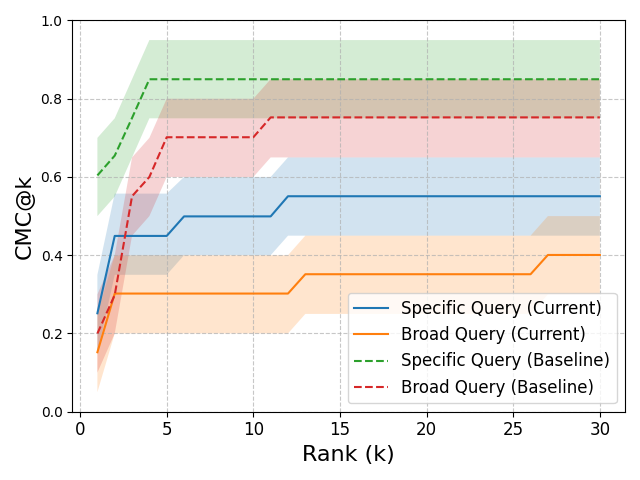
\includegraphics[width=\columnwidth]{fig/cmc.png}
    \caption{}
    \label{fig:cmc}
\end{figure}

\begin{table}[h]
\centering
\caption{Retrieval performance for specific and broad queries. Best results in bold.}
\begin{tabular}{l|c|c|c}
\toprule
\multicolumn{4}{c}{\textbf{Specific Queries}} \\
\midrule
\textbf{Method} & \textbf{Rank-1} & \textbf{Rank-5} & \textbf{mAP} \\
\midrule
Current  & 0.254 ± 0.097 & 0.450 ± 0.112 & 0.365 ± 0.093 \\
Baseline & \textbf{0.600 ± 0.110} & \textbf{0.850 ± 0.081} & \textbf{0.683 ± 0.091} \\
\midrule[0.8pt]
\multicolumn{4}{c}{\textbf{Broad Queries}} \\
\midrule
\textbf{Method} & \textbf{Rank-1} & \textbf{Rank-5} & \textbf{mAP} \\
\midrule
Current  & 0.150 ± 0.082 & 0.301 ± 0.103 & 0.231 ± 0.083 \\
Baseline & \textbf{0.199 ± 0.090} & \textbf{0.698 ± 0.103} & \textbf{0.369 ± 0.078} \\
\bottomrule
\end{tabular}
\end{table}






%------------------------------------------------


%------------------------------------------------

\section*{Discussion}
% Poudari da je evalvacija težka, ker delamo na unabeled data, in je treba ročno preverjati rezultate
In this project, we developed a conversational agent using Retrieval-Augmented Generation (RAG) to assist with academic research in automatic re-identification. Our approach aimed to enhance the language model's responses by integrating recent research papers from arXiv and CVF, focusing on improving retrieval relevance and accuracy. 
While the system showed promise in generating more informed responses, it also highlighted several challenges and areas for improvement.
One of the main challenges we faced was the difficulty of evaluating retrieval performance on unlabeled data. Since our queries were designed to retrieve specific papers, we had to manually verify the relevance of retrieved results, which is time-consuming and subjective. This limitation underscores the need for better evaluation protocols in RAG systems, particularly when dealing with specialized domains where labeled datasets may not be readily available.
Furthermore, while our enhanced retrieval pipeline utilized query rewriting and re-ranking strategies, it still struggled with retrieving the exact target papers in many cases. The issue might stem from the fact that the embedding model was trained on data, that resembled the raw abstracts, rather than the rewritten queries we used. This suggests that further fine-tuning of the embedding model, or using different model altogether could improve performance.



%----------------------------------------------------------------------------------------
%	REFERENCE LIST
%----------------------------------------------------------------------------------------
\bibliographystyle{unsrt}
\bibliography{report}


\end{document}
